\cleardoublepage
\mbox{}


\chapter{Tecnología Openvino}
\label{ch:chapter3}
Openvino es un conjunto de herramientas multi plataforma desarrollada por Intel que facilita la transición entre entre los entornos de entrenamiento y producción de nuestro modelo de aprendizaje profundo.
Openvino a pesar de estar desarrolalda por una empresa comercial como Intel peternece al conjunto de aplicaciones de código abierto, de modo que podemos visualizar su código fuente, repotar fallos en incluso realizar aportaciones.
Podemos visualizar el diseño y el código de la aplicación en su repositorio oficial de Github en el siguiente link https://github.com/openvinotoolkit/openvino.
El cometido principal de esta aplicación es la optimización del tiempo de inferencia de un modelo de deep learning previamente entrenado.
Para ello Openvino dispone de su propio formato de definición de modelos, son estos archivos los que procesa su propia red de inferencia multi plataforma, la cual está preparada para procesar estos archivos y poder
realizar los trabajos de manera concurrente, aprovechando así, toda la potencia de los procesadores o gpu actuales.


En la siguiente figura podemos observar el flujo de trabajo que se ha seguido en este trabajo haciendo uso de la herramienta Openvino~\ref{fig:Arquitectura de optimización de modelos con Openvino}
En primer lugar optimizaremos la topología de nuestro modelo a uno preparado para ser procesado por la red de inferencia de alto rendimiento de Openvino.
Finalmente nuestra red de inferencia será la que realice el trabajo de clasificación en el entorno de producción de nuestra aplicación

\begin{figure}
    \centering
    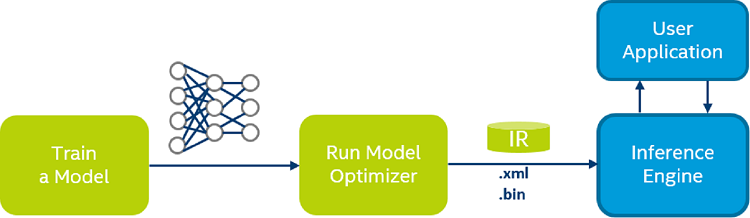
\includegraphics[width=0.8\textwidth]{images/chapter3/openvino_workflow.png}
    \caption{Arquitectura de optimización de modelos con Openvino}
    \label{fig:Arquitectura de optimización de modelos con Openvino}
\end{figure}


\section{Herramientas que lo componen}\label{sec:herramientas-que-lo-componen}
Esta tecnología desarrollada por intel se centra principalmente en la optimización de modelos de redes neuronales convolucionales para potenciar su velocidad de inferencia mediante las distintas herramientas que lo componen.
La herramienta soporta distintos hardwares como FPGA, Intel movidius, procesamiento por GPU\@ y también distintos sistemas operativos como Mac Os, Linux o Windows.
Las características principales de esta aplicación se resumen en dos puntos :
\begin{itemize}
    \item \textbf{Optimizador de modelos de deep learning}: Aplicación de interfaz de línea de comando, la cual usa como base modelos de frameworks populares como Caffe, TensorFlow, MXNet, Kaldi y ONNX para convertirlos a un modelo optimizado de Openvino.
    \item \textbf{Interfaz de inferencia de modelos de deep learning}: API de alto rendimiento multi plataforma para realizar la inferencia de manera rápida.
\end{itemize}

\subsection{Optimizador de modelos de deep learning}\label{subsec:optimizador-de-modelos-de-deep-learning}
Para poder realizar la optimización de nuestro modelo de deep learning previamente entrenado se necesita el binario que contiene la topología de la red del modelo.
Una vez el optimizador de Openvino recibe como argumento nuestro modelo realiza una conversión de cada capa interna de la red a una nueva capa.
Esta nueva capa, ya del formato de Openvino conserva los pesos de la red anterior, sin embargo, la definición de la misma está preparada para la que la aplicación de inferencia de Openvino pueda leerla correctamente.
Openvino proporciona de manera genérica distintos scripts para realizar esta conversión.
Se incluyen distintos scripts para los diferentes frameworks de deep learning más actuales, los mismos están codificados en python y podemos modificar su código fuente, aunque en principio no es necesario porque ya vienen preparados para funcionar.

\subsection{Interfaz de infernecia de modelos de deep learning}\label{subsec:interfaz-de-infernecia-de-modelos-de-deep-learning}
Con nuestro modelo y su topología convertida a un formato válido de Openvino tenemos todo lo necesario para poder realizar clasificaciones con la interfaz de inferencia de Openvino.
La optimización de inferencia se produce en este punto, donde cada capa de nuestro modelo original es procesada por la aplicación de inferencia en un lenguaje de bajo nivel, el cual está optimizado
para realizar operaciones vectoriales bajo total control del programador.
Este lenguaje es C++, aunque el programa puede ser utilizada también en Python gracias al uso de su API, la cual traduce las peticiones realizadas en Python al core de la interfaz, el cual es C++ puro.
Todas las capas usadas en este proyecto son compatibles de manera directa con las predefinidas por la interfaz de inferencia.
Openvino nos da la posibilidad de añadir capas personalizadas, con el inconveniente de que estas capas deben de ser programadas por el usuario de manera explícita en C++ para hacerlas compatibles con el resto de la aplicación y, por supuesto, mantener estas
nuevas capas a lo largo de las distintas actualizaciones y posibles cambios que pueda sufrir la aplicación.


\section{Conversión del modelo a la plataforma OpenVINO}\label{sec:conversión-del-modelo-a-la-plataforma-openvino}
Para realizar la conversión del modelo en primer lugar es necesaria la exportación del modelo original de tensorflow a un formato compatible con la red de optimización de modelos de Openvino.
La serialización por defecto de un modelo de tensorflow puede incluir de manera independiente :

\begin{itemize}
    \item Un punto de control TensorFlow que contiene los pesos del modelo.
    \item Un prototipo 'SavedModel' que contiene el grafico subyacente de Tensorflow.
    Separa los graficos que se guardan para prediccion (servicio), capacitacion y evaluacion.
    Si el modelo no se compilo antes, solo el grafico de inferencia se exporta.
    \item La configuracion de arquitectura del modelo, si esta disponible
\end{itemize}

Los métodos exactos para la serializaciñon del modelo varían según la versión de tensorflow, en cualquier caso la metodologíoa de conversión exacta utilizada
para este proyecto se puede encontrar en el repositorio de código fuente de este trabajo en Github : https://github.com/A-Ortiz-L/multispectral-imaging-cnn-final-degree-work
Este modelo de Openvino va a servir tanto de punto de partida para la optimización del mismo como para su uso directo en el servicio personalizado de tensorflow para desplegar
modelos en producción.
Una vez exportado el modelo de deep learning al formato estándar de tensorflow tendremos a nuestra disposición los ficheros necesarios para realizar la trasnformación de estos al formato de Openvino.
Para realizar esta operación se hace uso de la herramienta de Optimización de modelos, en concreto, con el script específico de tensorflow, cuyo nombre
es mo_tf.py.
Este código fuente es ejecutado en la línea de comandos del sistema operativo correspondiente con los siguientes parámetros de entrada en la línea de comandos :
\begin{lstlisting}
mo_tf.py --input_model model.pb --input_model_is_text -b 1
\end{lstlisting}
En este comando se epecifica mediante el flag --input_model_is_text que nuestro fichero no está codificado en código binario, por lo que es texto plano.
Esta opción es totalmente configurable y depende del proceso de exportación.
Se ha encontrado útil la opción de exportaciòn a texto plano ya que de esta manera
se puede observar la arquitectura de la red y los pesos pertenecientes a cad capa.



\section{Inferencias.
Tensorflow vs OpenVINO}\label{sec:inferencias.-tensorflow-vs-openvino}
(Los resultados no habría que ponerlos en teoría aquí, sino llevarlos al apartado